
\chapter{Introduction}
Power Electronics, especially converters, lead to a more complex electrical field stress in insulation systems of energy transmission systems as it introduces pulses (>1 kV) with high slew rates and high repetition frequencies (> 1 kHz) superimposed on low frequencies or DC. Latter can cause a partial discharge (PD) in the insulation system, i.e. a transient breakdown of a part of the insulation system. \cite{TransformerEngineering}. However, there are already effects below partial discharge that are not well investigated yet. They do as well result in an accelerated aging of the insulation due to the sustained repetition of the converter pulses. 
\newline


\begin{figure}[!ht]
  
  
  \centerline{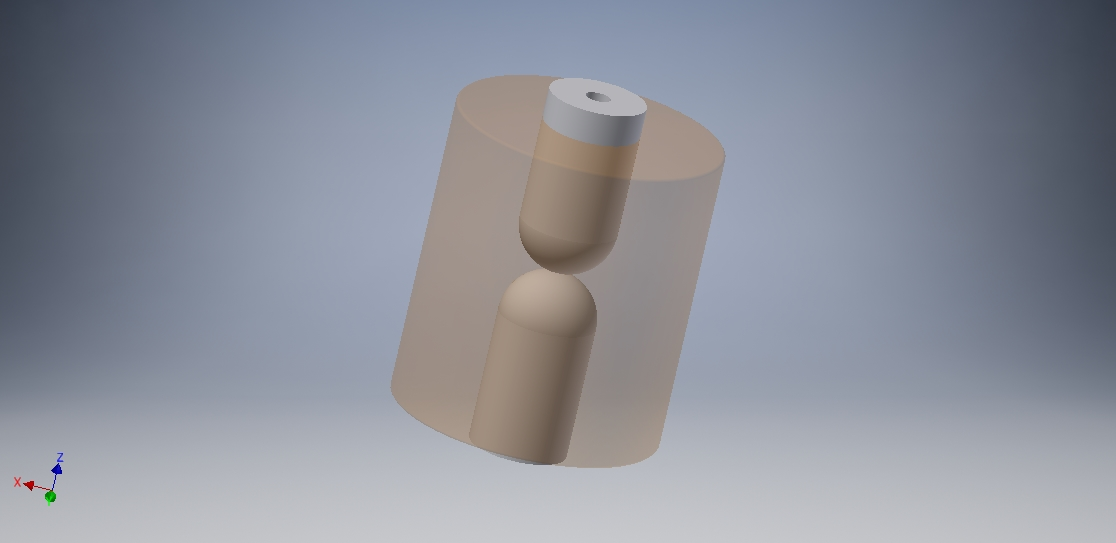
\includegraphics[width=0.5\textwidth]{figures/intro/epoxy_specimen.jpg}}
\caption{Epoxy specimen used for measurements of the partial discharges. \protect\footnotemark}
	\label{fig.specimen}
\end{figure}

In a new approach, a quantification of the pre-breakdown modification should be obtained with the use of an online moitoring the dielectric permittivity for several harmonics \cite{FaerberMVISS}.
The first part of this semester project is aimed at getting the dielectric permittivity by measuring the capacity of the specimen shown in figure \ref{fig.specimen}. When using a specimen for the first time it is assumed that it's dielectric permittivity is always the same. In order to be able to determine the distance of the two electrodes a reference measurement is made and a look-up-table is created. 

The second part of the project is the investigation of the suitability of current transformers in dielectric spectroscopy. For measuring very small below-PD currents it is doubted that a current transformer does not deteriorate the signal in a way that an acceptable measurement is possible. The results of this work, however, indicate that the use of a current transformer does deteriorate the guess of $\epsilon$ significantly. 

\footnotetext{{CAD provided by Raphael R\"arber}}
